\subsubsection{Language}

At the beginning of the project, C++ was chosen to code the software. This is for simple reasons: C++ being compiled, it is runs faster so it's more indicated than Java to create an efficient algorithm.  Moreover it has several complete graphical libraries, like \emph{Qt} and \emph{SFML}, so it's easy to create the graphical interface that will be needed for the project.

\subsubsection{Software}

The software used to develop the project has already been chosen. The coding will be realized on \emph{Microsoft visual studio 2013}, and the version manager will be git. These two softwares are used a lot in the industry so we have to be familiar with them.
For the bibliography, Zotero will be used as it allows for the creation of .bib files, the bibliographic format use by LaTeX.

\subsubsection{Grid5000}

Grid5000 is a French cluster of computers that links a lot of computers from different research centers. Some of this machines have, in addition of a good CPU, a NVIDIA Tesla GPU that could be use to parallelize the \emph{MCTS}. Of Course use this cluster will require some specific parallelization that will be introduced in the next part.

\subsubsection{Parallelization}

\paragraph{Multi cores parrelization}\mbox{}\\\mbox{}\\

OpenMp is a very simple and efficient API\footnote{Application Programming Interface} that supports parallelization. It consists some pre-compilation instructions, with only a few lines of code. It allows to obtain a parallel version of the algorithm. As it can be seen in the figure \ref{fig:OpenMp}, it uses a large part of shared memory which allows a quick and efficient communication between the different threads. But it's not designed for using a cluster of computers, because the memory access will not be efficiant for computers which are far away. But there is a method to avoid this problem that is addressed later.
\begin{figure}[!h] 
\centerline{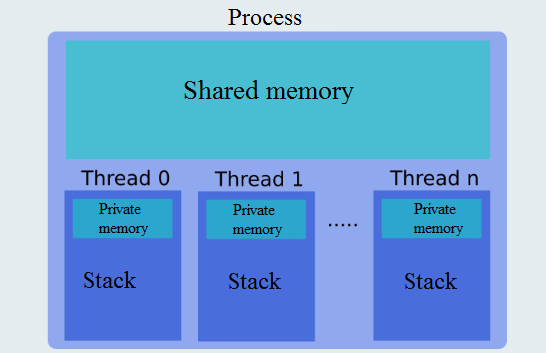
\includegraphics[scale=0.50]{3_Software_considered/MultithreadingMP_boost_Visual_MPI_5000_Zotero_Project_Baptiste/OpenMP}}
   \caption{\label{étiquette} OpenMp : memory management}
\label{fig:OpenMp}
\end{figure}
\newpage
\paragraph{Computer parallelization}\mbox{}\\\mbox{}\\

MPI is a more complex method of parallelization than openMp but it is more complete. In addition to using several cores on a single machine, MPI can also be used to design software that uses a cluster of machines. As it can be seen in the figure \ref{fig:MPI}, it doesn't use shared memory, all the data of the threads are duplicated at their creation. It uses signals to permit the communication between the threads. One of its advantages is that it makes possible to use multiple computers: as the data is duplicated, there isn't the problem of time to access the memory. But attention is to be paid for the cost of communication between the threads, as if too many signals are used, the time that was gained using the parallelization will be lost. It's adapted for tree parallelization, because the only things to be done are to duplicate the data at the beginning and return the result at the end of the assigned time.

\begin{figure}[!h] 
\centerline{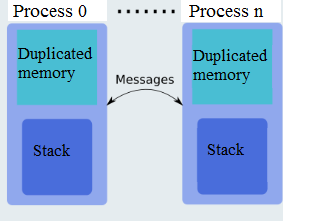
\includegraphics[scale=0.85]{3_Software_considered/MultithreadingMP_boost_Visual_MPI_5000_Zotero_Project_Baptiste/MPI}}
   \caption{\label{étiquette} MPI : memory management}
\label{fig:MPI}
\end{figure}

\paragraph{Hybrid parallelization}\mbox{}\\\mbox{}\\

As stated before, openMp and MPI have their respective pros and cons, but their respective problems can be tackled by using both. That means MPI can be used to dispatch the work onto the different computers and openMp can be used to divide it on the different threads of each machine. This can permit the use of multiple parallelization strategies, for example tree parallelization between the machines and leaf or root parallelization on each machine. Also, it reduces the amount of code needed to manage the threads. It also means that as the interaction between the threads is reduced, to maximize parallelization.

\paragraph{Boost Library}\mbox{}\\\mbox{}\\

Boost is a well known library for C++ which permits the management of threads, amongst other things. Basically, it can only be used for one computer but it also covers socket handling which makes parallelization between several machines easier. It also holds tools for graph modelisation that can improve a lot the efficiency of the algorithms.

\paragraph{GPU implementation}\mbox{}\\\mbox{}\\

During the research, it was observed that efficiancy of the \emph{MCTS} algorithm improves by using GPU. As Kamil Rocki said in his thesis "Large Scale Monte Carlo Tree Search on GPU"\cite{GPU} , one GPU's performance is equivalent to 50 CPU threads. But this implementation is not perfect, in fact that GPU possess very less cache memory, so if the data model is too big the parallelization will be inefficient. Also the trees that it creates will be less deep than those of a CPU, but when a CPU can develop two branches, a GPU will be developing hundreds of branches simultaneously. Another thing that is to be kept in mind is that a GPU can switch to another thread immediately without any cost of context switching. 

Some machines from Grid5000 have NVIDIA GPUs, so one of the possibilities is to use hybrid parallelization as it was described previously by using MPI (or boost library) and openAcc (an equivalent of openMp which allows the use of the GPU) or CUBA (a framework for GPU parallelization develop by NVIDIA). This way, bigger trees will be developed and give a better solution than when using only the CPU, even if the branches are less deep.